\documentclass[12pt]{article}

% Modelo de artigos da Sociedade Brasileira de Computacao (SBC).
\makeatletter
\def\input@path{{latex/}}
\makeatother
\usepackage{sbc-template}
\usepackage{graphicx,url}
\usepackage[T1]{fontenc}
\usepackage[brazil]{babel}
\usepackage{amsmath}
\usepackage{array}
\usepackage{flafter}
\usepackage{float}
\usepackage{placeins}

% Template SBC sem alterações de formatação: corpo do texto e bibliografia
% seguem o padrão original (sbc-template.sty). Os floats são ancorados no
% ponto de citação com [H] (pacote float, já carregado).
% Pontos de quebra para o nome do corpus, que o TeX não hifeniza sozinho e
% recorrentemente deixa estourar a linha. Não altera a formatação do template.
\hyphenation{Fig-sha-re}
\setlength{\intextsep}{6pt plus 2pt minus 2pt}
\setlength{\abovecaptionskip}{4pt}
\setlength{\belowcaptionskip}{4pt}
% O template usa \flushbottom, que estica o espaço vertical entre parágrafos
% para igualar a altura das páginas e abre vãos visíveis. O texto usa
% \raggedbottom: cada página termina onde o conteúdo termina, sem esticar.
\raggedbottom


\newcommand{\pendente}[1]{\textbf{[PENDENTE: #1]}}

\title{BrainSniffer: uma CNN compacta e causal para estimar a referência BIS a partir de EEG frontal}

\author{Bruno Rocha Guimarães\inst{1}\and Igor Gonzales Pimenta\inst{1}\and José Garcia Vivas Miranda\inst{1}}

\address{Ciência da Computação -- Centro Universitário Jorge Amado\\
  Salvador, Bahia -- Brasil}

\begin{document}

\maketitle

\begin{abstract}
BrainSniffer is a compact, causal convolutional network that estimates a Bispectral Index (BIS) reference label from frontal electroencephalography (EEG), designed so that its processing chain can run in real time. It uses five-second windows at 128 Hz, 0.15M parameters, ten training epochs, and partitions grouped by case or subject, so no case crosses partitions. On a five-case Figshare holdout the active checkpoint reached mean absolute error (MAE) 7.03 against 8.86 for a spectral baseline, with ordinal prediction probability (Pk) 0.773; on 15 VitalDB cases the same checkpoint degraded to 12.43 with Pk 0.515, indistinguishable from chance, a collapse the spectral baseline reproduces. A causal per-case exponential smoothing (EWMA, applied to frozen predictions, no retraining) is the whole of its temporal machinery and brings the mixed candidate to 5.84 MAE on Figshare, the same order of magnitude as a published TCN-BiLSTM reporting 6.03 $\pm$ 0.38 with seven times more parameters (protocols differ, so this is not a ranking); the gain does not transport to VitalDB (7.89). These results are retrospective and exploratory, and the ten-point BIS reference is a reading scale, not evidence of equivalence, acceptability or non-inferiority. BrainSniffer neither measures consciousness nor supports clinical decisions, alarms, or drug dosing.

\textbf{Keywords:} frontal EEG; BIS reference label; compact convolutional network; grouped validation; domain shift; causal smoothing; deployability.
\end{abstract}

\begin{resumo}
O BrainSniffer é uma rede convolucional compacta e causal que estima, a partir de eletroencefalografia (EEG) frontal, um rótulo de referência do Índice Bispectral (BIS), projetada para que sua cadeia de processamento possa rodar em tempo real. Ela usa janelas de cinco segundos a 128 Hz, 0,15M de parâmetros, dez épocas de treino e partições agrupadas por caso ou pessoa, de modo que nenhum caso cruza partições. Em cinco casos Figshare, o checkpoint ativo obteve erro absoluto médio (MAE) 7,03 contra 8,86 de um baseline espectral, com probabilidade de predição $P_K$ 0,773; nos 15 casos VitalDB, o mesmo checkpoint degradou para 12,43 com $P_K$ 0,515, indistinguível do acaso, colapso que o baseline espectral reproduz. Uma suavização exponencial causal por caso (EWMA, aplicada a predições congeladas, sem retreino) é toda a sua maquinaria temporal e leva o candidato misto a 5,84 de MAE no Figshare, na mesma ordem de grandeza de um TCN-BiLSTM publicado que reporta 6,03 $\pm$ 0,38 com sete vezes mais parâmetros (os protocolos diferem; não é um ranking); o ganho não transporta para o VitalDB (7,89). Os resultados são retrospectivos e exploratórios, e a referência de dez pontos BIS é escala de leitura, não evidência de equivalência, aceitabilidade ou não-inferioridade. O BrainSniffer não mede consciência nem apoia decisão clínica, alarme ou dose.

\textbf{Palavras-chave:} EEG frontal; rótulo BIS; rede convolucional compacta; validação agrupada; deslocamento de domínio; suavização causal; implantabilidade.
\end{resumo}

\section{Introdução}

Na anestesia geral, é preciso saber se o paciente está suficientemente hipnotizado sem exagerar na dose, e para isso usam-se referências objetivas de profundidade. O Índice Bispectral (Bispectral Index, BIS), calculado a partir da eletroencefalografia (EEG) frontal, é a referência mais usada à beira do leito, mas é uma saída proprietária: sua regra de combinação não é publicada e não pode ser reproduzida exatamente a partir do sinal. Redes convolucionais 1-D são uma escolha usual para sinais fisiológicos de baixa dimensão \cite{kiranyaz2021,craik2019}, e modelos desse tipo já tentaram aproximar esse rótulo; eles enfrentam ainda um risco metodológico silencioso: janelas vizinhas da mesma cirurgia são quase idênticas, então uma partição aleatória entre treino e teste mede o reconhecimento de casos já vistos, não a generalização. Falta um estimador compacto e causal, avaliado com partições por caso e contra um controle espectral entre fontes: este trabalho apresenta o BrainSniffer.

A pesquisa responde a três perguntas. (i) Uma rede neural convolucional unidimensional compacta (1-D CNN), sob validação agrupada, aproxima o rótulo BIS na faixa de variabilidade do próprio monitor e supera um controle mais simples baseado em medidas espectrais (baseline espectral)? (ii) Esse desempenho é competitivo com o de um modelo contemporâneo várias vezes maior, sem abrir mão de uma cadeia que possa ser exportada para uso ao vivo? (iii) Ele se mantém ao trocar a fonte dos dados, do Figshare para o VitalDB, com outro equipamento, montagem e população? O objetivo geral é responder às três com métricas primárias escolhidas de antemão (o MAE por janela, ancorado na variabilidade do próprio monitor, e a probabilidade de predição $P_K$, que mede a ordenação). As demais métricas e análises são secundárias.

Vale fixar o vocabulário: o modelo estima um rótulo de referência derivado do BIS, não o BIS como grandeza independente, pois o BIS é a saída de um monitor sobre o mesmo sinal. A contribuição é uma cadeia compacta e causal, avaliada com partições por grupo e contra um controle espectral, que atinge a variabilidade do monitor no corpus de origem e fica na mesma ordem de grandeza de um modelo contemporâneo sete vezes maior, ao custo de não transportar para outra fonte; o escopo não é desenvolver um dispositivo médico.





\section{Fundamentação e trabalhos relacionados}

\subsection{O índice BIS e seus limites}

% Quebra de linha local (sem alterar o texto).
\begingroup\emergencystretch=1em\relax Sob anestesia geral, o EEG frontal desacelera e ganha amplitude, com alfa frontal e ondas lentas \cite{purdon2015}. O Índice Bispectral (BIS) é uma saída proprietária do EEG frontal, em escala de 0 a 100, com a faixa intermediária como referência de hipnose \cite{johansen2000}. O cálculo combina características temporais, espectrais e bispectrais por regra não publicada; por ser fechado, não pode ser reproduzido do EEG. O BIS é só auxílio sob supervisão, não medida de consciência ou dose. Sua leitura varia com EMG, fármacos e atrasos \cite{schuller2015,hans2005,pilge2006}, e ensaios guiados tiveram resultados dependentes do comparador \cite{baware,bunaware,bagrecall}. O BIS chega suavizado e com atraso \cite{pilge2006}, e a suavização causal é prática comum no corpus \cite{sukriti2026}.
\par\endgroup

\subsection{Vazamento entre janelas e partição por grupo}

Redes profundas já foram estudadas com alvos, canais, populações e equipamentos distintos para aproximar índices derivados de EEG \cite{park2020,shi2023}. O problema é que janelas vizinhas da mesma cirurgia são parecidas entre si em amplitude, espectro e nível de BIS, porque refletem o mesmo paciente no mesmo plano anestésico. Se essas janelas forem espalhadas aleatoriamente entre treino e teste, o teste contém trechos quase idênticos aos de treino: é o vazamento (\textit{leakage}), que infla o desempenho. Para evitá-lo, os dados são separados por caso ou pessoa (o grupo), ao custo de uma estimativa mais pessimista e mais realista para um caso novo \cite{sukriti2026,saeb2017}.

\subsection{Corpora, transparência e relato de modelos}

O conjunto ``EEG and BIS raw data'' reúne 24 casos anônimos com EEG frontal e valores BIS, publicado no repositório Figshare sob licença CC BY 4.0 \cite{ma2017}. Um estudo anterior no mesmo corpus usou características multiescala com análise discriminante linear (LDA) e sustenta a descrição do corpus, mas não é evidência de rede convolucional \cite{nsugbe2022}. Outros estudos estimaram a concentração anestésica derivada de EEG com cadeia dedicada e o índice de estado do paciente (Patient State Index, PSI) com quatro canais em 18 idosos sedados; ambos demonstram viabilidade em configurações específicas, sem comparabilidade direta com o rótulo, o canal ou a população deste trabalho \cite{park2020,shi2023}.

O VitalDB é um banco de sinais perioperatórios de milhares de cirurgias e inclui os canais de EEG frontal e de BIS usados aqui \cite{lee2022,vitaldb}. O conjunto aberto exige licença CC BY-NC-SA 4.0 e acordo de uso de dados, sem redistribuição. Escala, equipamento, montagem e população diferem do Figshare; o VitalDB informa a sensibilidade à troca de fonte, sem isolar a causa. O rótulo também difere no instrumento: BIS a cada 5 s por sensor BIS Quatro no Figshare \cite{ma2017,sukriti2026} contra BIS de 1 s de monitores BIS Vista no VitalDB \cite{vitaldb,lee2022}, com algoritmo e suavização não públicos. O DOSE-I não foi incorporado por usar escala observacional MOAA/S, não conversível em BIS \cite{dosei}.

Uma reimplementação aberta do algoritmo do índice não torna um regressor treinado contra o BIS equivalente a um monitor \cite{openbis}. Independência entre desenvolvimento e avaliação, descrição de grupos e análise de acordo e calibração são centrais no relato de modelos \cite{tripodai,archer2021}.

\section{Materiais e métodos}

A Tabela~\ref{tab:modelos} resume os dois checkpoints e a Figura~\ref{fig:pipeline} o fluxo retrospectivo: o ``ativo'' foi ajustado só no Figshare e testa o limite interno e a queda ao mudar de corpus; o ``misto'' viu também parte do VitalDB, de modo que seu desempenho nessa fonte não mede transporte para fonte nova.

\begin{table}[H]
\centering
\small
\begin{tabular}{p{0.25\columnwidth}p{0.29\columnwidth}p{0.37\columnwidth}}
\hline
Modelo & Treinado com & Avaliado em\\
\hline
Modelo A -- Figshare (ativo) & Figshare & Figshare (holdout por caso) e VitalDB (avaliação cruzada de dataset)\\
Modelo B -- misto & Figshare + parte do VitalDB & Figshare (benchmark histórico) e VitalDB (holdout histórico por participante)\\
\hline
\end{tabular}
\caption{Definição conceitual dos dois checkpoints.}
\label{tab:modelos}
\end{table}

\begin{figure}[H]
\centering
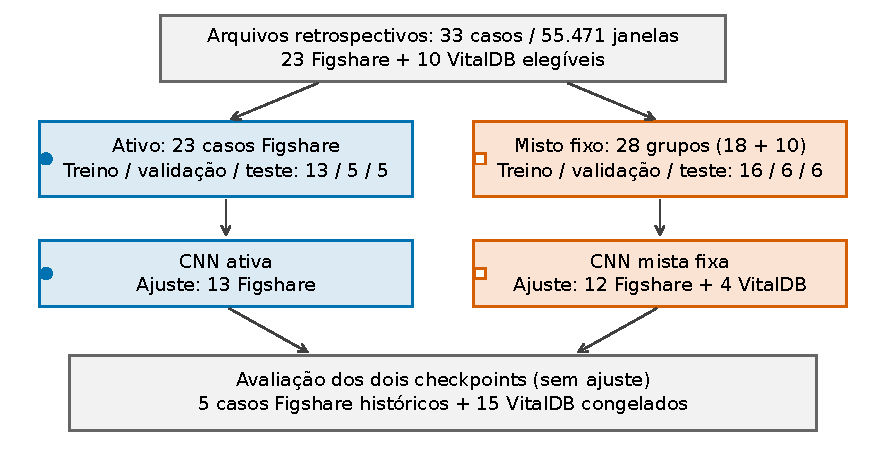
\includegraphics[width=0.92\columnwidth]{figures/pipeline.pdf}
\caption{Fluxo retrospectivo auditável do BrainSniffer.}
\label{fig:pipeline}
\end{figure}

\subsection{Fontes, unidades de agrupamento e partições}

Cada arquivo é uma gravação inteira, tratada como um caso; de cada caso saem janelas de 5 s, unidades de treino e de métrica. O grupo é a unidade que nunca cruza partições. O corpus tem 59 arquivos: 44 no pool de desenvolvimento e 15 casos VitalDB congelados. Após os gates de qualidade, 23 casos Figshare e dez VitalDB ficaram elegíveis (33 casos, 55.471 janelas). No Figshare não há identificador de participante; no VitalDB o agrupamento usa o identificador e reúne reoperações \cite{ma2017,lee2022}.

O ativo usou os 23 Figshare elegíveis (13/5/5 com seed 42). O misto fixo excluiu o holdout Figshare e usou 18 grupos Figshare mais dez VitalDB (28 grupos, 49.948 janelas; ajuste com 12 Figshare e quatro VitalDB). Só o teste interno é lido como resultado; as janelas de validação não aparecem nas tabelas.

Os mesmos cinco Figshare (casos 3, 4, 5, 9 e 19) servem aos dois checkpoints. Para o misto, os 15 VitalDB (arquivos 1--17, sem 11 e 15, que não têm os tracks requeridos) vêm da mesma fonte do desenvolvimento e já haviam sido inspecionados: é um holdout histórico após exposição ao domínio, não validação externa confirmatória \cite{tripodai}.

\subsection{Tarefa, pré-processamento e qualidade}

Cada exemplo é um trecho curto de EEG frontal em microvolts: 640 amostras, isto é, uma janela de 5 segundos amostrada a 128 Hz, com passo de 5 s na construção offline. Para cada início $t$, o alvo corresponde a $t+\mathrm{offset}$ (offset padrão 0 s), arredondado ao intervalo do BIS do caso. A Figura~\ref{fig:eeg} mostra duas janelas reais do caso 19 antes e depois do pipeline causal: um trecho limpo (pico de 38 $\mu V$, BIS 30) quase não muda (pico processado de 36 $\mu V$), enquanto um trecho com pico de 125 $\mu V$ (BIS 75) é contido para 88 $\mu V$ pelo clip, filtro e escala. O pipeline mantém a banda de 0,5--45 Hz, notch de 50 Hz de quarta ordem e a escala registrada (clip $\pm100\,\mu V$, divisor $50\,\mu V$); o filtro usa só passado e presente (estado causal por caso), com rota de fase zero apenas para análise offline \cite{ma2017,nsugbe2022}. O painel (c) mostra que, nesse caso, a potência relativa em teta cai quando o BIS sobe e a de beta e gama sobe junto, relação que o modelo explora; as lacunas brancas são quedas de eletrodo rejeitadas pelos gates.

\begin{figure}[H]
\centering
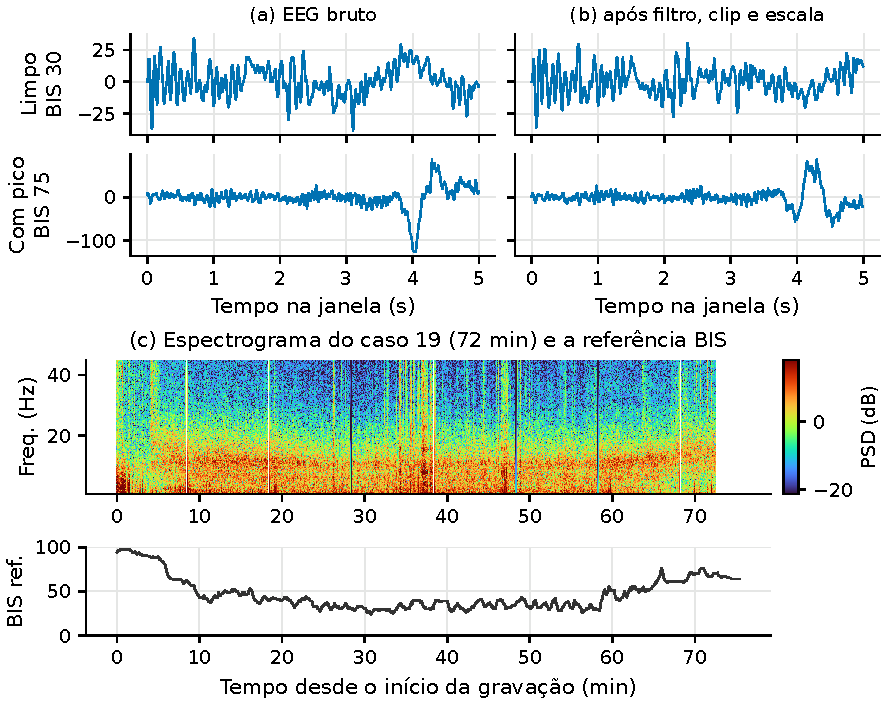
\includegraphics[width=0.95\columnwidth]{figures/eeg_windows.pdf}
\caption{Janelas reais do caso 19 e espectrograma da gravação. (a,b) Linha de cima, trecho limpo (BIS 30); linha de baixo, trecho com pico (BIS 75). Coluna da esquerda, sinal bruto; da direita, após clip, filtro causal e escala; o pico de 125 $\mu V$ é contido para 88 $\mu V$. (c) Espectrograma causal dos 72 min, na base de tempo da referência BIS; as faixas brancas são as quedas de eletrodo.}
\label{fig:eeg}
\end{figure}

Os gates exigem 90\% de EEG finito, lacuna máxima de 2 s, qualidade global 0,35, 80\% de BIS válido e 0,20 por janela (heurísticas sem calibração clínica; o Figshare 24 está em quarentena). Nos 15 VitalDB do benchmark, a construção offline interpola não finitos (podendo usar amostras futuras) e interpola o BIS para grade de 1 s sem máscara persistida: difere da rejeição do replay e limita a interpretação, mas foi mantida por fidelidade histórica.

\subsection{Modelos e treinamento}

A CNN histórica recebe a janela de 640 amostras em um canal, é treinada com perda Smooth L1 e tem saída sigmoidal escalada para $[0,100]$. Os braços novos do experimento fatorial (Seção~\ref{sec:fatorial}) usam perda de Huber com $\delta=5$, treino de até 120 épocas e normalização por sujeito, mantida a mesma arquitetura. A Tabela~\ref{tab:config} explicita a arquitetura e os parâmetros registrados no protocolo, sem carregar pesos. Recursos posteriores do treinador e arquiteturas opcionais não são atribuídos retroativamente a esses pesos.

\begin{table}[H]
\centering
\footnotesize
\begin{tabular}{p{0.28\columnwidth}p{0.63\columnwidth}}
\hline
Item & Configuração registrada\\
\hline
Convolucionais & Canais 1$\to$32$\to$64$\to$128$\to$128; \textit{kernel} 7, 7, 5, 5; \textit{padding} 3, 3, 2, 2; \textit{stride} 1; normalização em lote + GELU\\
\textit{Pooling} e cabeça & max-pooling de fator 2 nos 3 primeiros blocos; pooling médio global; camada densa 128--64--1, GELU, \textit{dropout} 0,20\\
Treino (ambos) & 10 \textit{epochs}, \textit{batch} 128, \textit{lr} $10^{-3}$, \textit{wd} $10^{-4}$, \textit{seed} 42; validação/teste: 20\% dos grupos em cada partição\\
Amostragem & Misto: balanceada por grupo/fonte; ativo: não registrada\\
Amplitude e \textit{notch} & \textit{Clip} $\pm100\,\mu V$, divisor de escala $50\,\mu V$, saída em $[-5,5]$; \textit{notch} 50 Hz, Q=30\\
\textit{Random Forest} & 100 árvores, profundidade máxima 12, mínimo de 2 amostras por folha, semente 42\\
\hline
\end{tabular}
\caption{Configuração histórica dos checkpoints.}
\label{tab:config}
\end{table}

A arquitetura compacta permite replay em CPU, sem superioridade presumida sobre alternativas \cite{park2020,shi2023}.

Como controle simples, o baseline espectral resume cada janela de 5~s em 14 atributos clássicos: potências absoluta e relativa das bandas delta (0,5--4 Hz), teta (4--8 Hz), alfa (8--13 Hz), beta (13--30 Hz) e gama (30--45 Hz), frequência de borda espectral em 90\% (SEF90), entropia espectral, valor eficaz (RMS) e \textit{line length}. Uma floresta aleatória (Tabela~\ref{tab:config}) é ajustada nas mesmas 15.894 janelas de treino e avaliada nas mesmas 5.523 de teste do holdout Figshare, com a mesma proteção contra vazamento. Se poucas medidas de espectro já alcançam erro parecido, a complexidade da CNN precisa ser justificada.

\subsection{Métricas, incerteza e análises exploratórias}

O desfecho primário é o MAE agregado por janela (casos longos pesam mais) e o de ordenação é a probabilidade de predição $P_K$ de Smith, Dutton e Smith \cite{smith1996}, detalhada na Seção~\ref{sec:pk}; as demais métricas são secundárias, sem correção para multiplicidade. Foram calculados RMSE, viés, Pearson e CCC de Lin para o rótulo contínuo, além de acurácia e macro-F1 em quatro faixas ($[0,40)$, $[40,60)$, $[60,80)$, $[80,100]$), lidas com rótulos curtos só para comunicação, sem validar limiar clínico \cite{tripodai}. Pearson mede associação, não acordo; a concordância usa inclinação de calibração, limites de concordância, ICC(2,1) e fração de $|erro|\leq10$, tudo exploratório. O $P_K$ e o Pearson agregados empilham todas as janelas (pares entre casos distintos entram na conta); por isso a Seção~\ref{sec:resultados} traz também mediana e amplitude por caso. A incerteza usa bootstrap de casos inteiros ($B=1.000$, seed 42, percentis 2,5/97,5), reamostrando o caso como unidade; com cinco casos Figshare, é exploratória (1.000 réplicas não equivalem a 1.000 casos) \cite{field2007,archer2021}.

Como referência externa, estudos que comparam montagens e interfaces do próprio BIS em neurocirurgia usam diferenças de até 10 unidades entre medições como critério de concordância \cite{dahaba2010,shiraishi2004,harada2021}. Esses estudos não definem uma variabilidade geral do monitor; a régua de 10 pontos é adotada aqui apenas como escala de leitura, não como limiar clínico nem critério de aprovação.

A comparação VitalDB também foi calculada por caso, pareando as janelas de cada caso. Uma análise de sensibilidade reaplicou o checkpoint ativo aos mesmos cinco casos Figshare, sem retreino, em uma grade de offset de $-20$ a $+20$ s; como a grade foi examinada após o treinamento, ela formula hipótese sobre alinhamento e não escolhe o atraso do rótulo \cite{pilge2006}.

\subsection{Replay, trajetória ilustrativa e suavização causal}

Replay é percorrer uma gravação existente (buffer de 5 s, atualização a cada 1 s), sem EEG físico. Para visualizar o comportamento temporal, fixou-se antes da inferência o caso 19 do holdout (4.355 s), com a configuração do checkpoint ativo em CPU, sem treino; a curva bruta posiciona-se no instante do alvo offline, sem representar disponibilidade sem atraso.

Como o alvo é uma saída já suavizada pelo monitor, o pipeline também permite uma média móvel exponencial causal por caso (EWMA), aplicada às predições congeladas, sem retreino: $s_t = \alpha y_t + (1-\alpha)s_{t-1}$, com $\alpha = 2/(\mathrm{span}+1)$ e reinício por caso; o \textit{span} é medido em janelas de 5 s. Usar apenas amostras passadas mantém o caminho compatível com o replay; a varredura de spans é retrospectiva e exploratória, e segue a prática de suavização temporal de trabalhos contemporâneos \cite{sukriti2026} e o atraso documentado do próprio índice \cite{pilge2006}.

\section{Resultados}
\label{sec:resultados}

\subsection{MAE: a CNN compacta supera o controle espectral}
\label{sec:mae}

O desfecho primário é o MAE agregado por janela. No holdout Figshare do checkpoint ativo, cinco casos e 5.523 janelas produziram MAE 7,03; o baseline espectral, na mesma partição, ficou em 8,86. No bootstrap pareado por caso, o $\Delta$MAE favorável à CNN é $-1{,}84$ (IC 95\% $-2{,}37$--$-0{,}66$): os intervalos excluem zero, mas com cinco casos o teste é exploratório. A Tabela~\ref{tab:figshare-baseline} resume o agregado, e a Tabela~\ref{tab:benchmarks} estende a comparação aos dois benchmarks e aos dois checkpoints.

\begin{table}[H]
\centering
\begin{tabular}{lrrrrr}
\hline
Modelo & MAE & RMSE & Pearson & Acurácia & Macro-F1\\
\hline
CNN ativa & 7,03 & 11,08 & 0,784 & 0,585 & 0,548\\
Baseline espectral & 8,86 & 13,23 & 0,667 & 0,540 & 0,480\\
\hline
\end{tabular}
\caption{Holdout Figshare comum (5 casos, 5.523 janelas; MAE e RMSE em pontos BIS).}
\label{tab:figshare-baseline}
\end{table}

A Figura~\ref{fig:trajectory} mostra o comportamento no caso 19, usado como ilustração: a CNN acompanha a queda inicial e a elevação final, mas superestima o patamar intermediário e não reproduz várias oscilações da referência. Nas 850 janelas aceitas, MAE 8,72, viés $+4{,}79$ e Pearson intra-caso 0,910: associação alta não elimina erro sistemático, e o caso é exemplo ilustrativo, não evidência de generalização.

\begin{figure}[H]
\centering
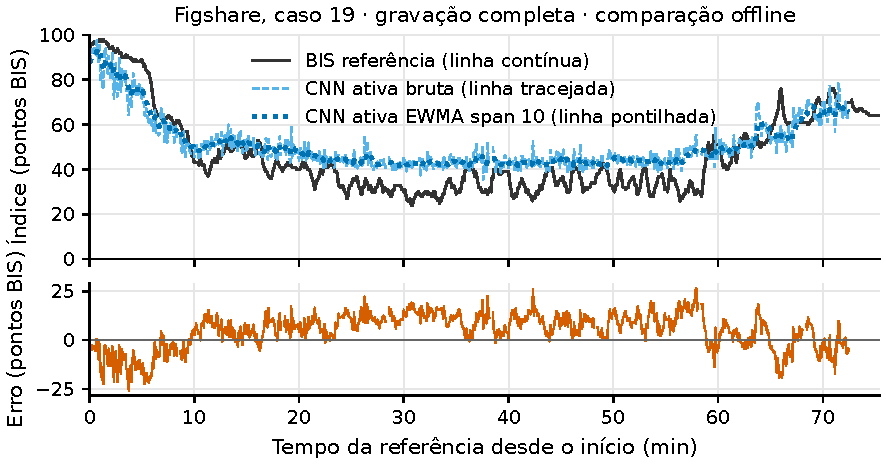
\includegraphics[width=0.95\columnwidth]{figures/bis_trajectory.pdf}
\caption{Trajetória offline do caso 19: referência e predição bruta (topo) e erro por janela (base).}
\label{fig:trajectory}
\end{figure}

\begin{table}[H]
\centering
\footnotesize
\setlength{\tabcolsep}{1pt}
\begin{tabular}{llrrr}
\hline
Benchmark & Modelo (fontes vistas) & MAE (IC 95\%) & Pearson (IC 95\%) & $P_K$ (IC 95\%)\\
\hline
Figshare & ativo (Figshare) & 7,03 (6,38--8,24) & 0,784 (0,703--0,881) & 0,773 (0,679--0,828)\\
Figshare & misto (Figshare+VitalDB) & 6,69 (5,65--8,53) & 0,818 (0,751--0,890) & 0,774 (0,676--0,835)\\
VitalDB & ativo (Figshare) & 12,43 (11,05--14,45) & 0,024 ($-0{,}126$--0,193) & 0,515 (0,434--0,581)\\
VitalDB & misto (Figshare+VitalDB) & 8,60 (7,57--9,95) & 0,688 (0,606--0,752) & 0,672 (0,591--0,737)\\
VitalDB & RF espectral & 13,62 (11,98--16,01) & $-0,036$ ($-0,162$--0,111) & 0,502 (0,447--0,551)\\
\hline
\end{tabular}
\caption{Comparação retrospectiva nos benchmarks históricos; 5 casos no \mbox{benchmark} Figshare e 15 no VitalDB; MAE em pontos BIS; IC 95\% por bootstrap agrupado por caso; o RF espectral viu apenas o Figshare.}
\label{tab:benchmarks}
\end{table}

Três dos quatro MAE dos checkpoints (Tabela~\ref{tab:benchmarks}) ficam abaixo de 10 pontos, a escala de leitura adotada \cite{harada2021}, que dá escala ao número sem funcionar como critério de aprovação. Só o ativo no VitalDB (12,43) a ultrapassa. O misto reduz o MAE nos dois benchmarks (6,69 e 8,60), mas no Figshare a diferença frente ao ativo não é sustentada ($\Delta$MAE pareado $0{,}34$, IC $-0{,}28$--$0{,}81$), e o ganho no VitalDB vem de um candidato que já viu essa fonte: é adaptação após exposição ao domínio, não transporte para fonte nova.

A fronteira está no transporte. O checkpoint que fica em 7,03 no Figshare vai a 12,43 no VitalDB, e o baseline espectral reproduz o colapso (13,62, com $P_K$ 0,502): a perda não é específica da CNN nem do seu treino. A Figura~\ref{fig:comparison} detalha a comparação pareada por caso, em que o misto melhora 14 dos 15 casos VitalDB ($\Delta$MAE $+3{,}83$, IC $2{,}95$--$4{,}94$), com piora de cerca de 0,67 ponto no caso 16. A leitura pareada evita que cirurgias longas dominem e revela heterogeneidade: 14 acertos contra 1 piora convivem com margens pequenas.

\begin{figure}[H]
\centering
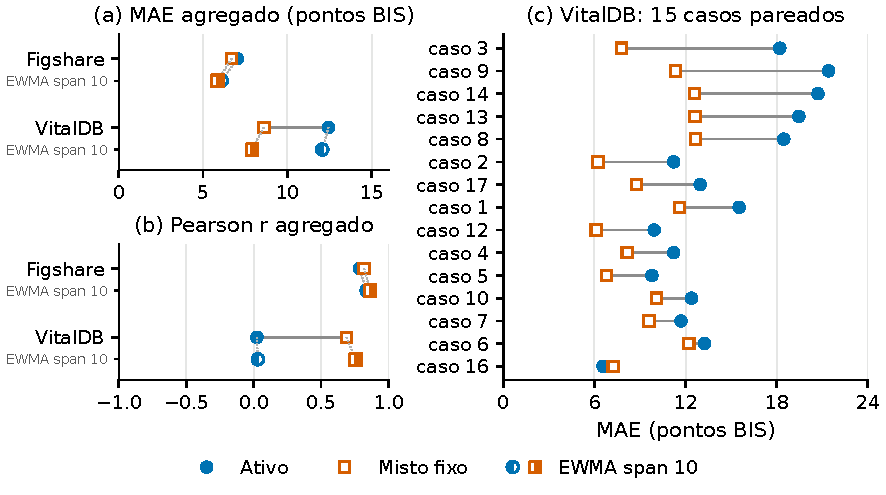
\includegraphics[width=0.95\columnwidth]{figures/comparison.pdf}
\caption{Agregados por janela e MAE pareado por caso; em (c), cada ponto é um caso e linhas à esquerda indicam menor MAE do misto.}
\label{fig:comparison}
\end{figure}

\subsection{$P_K$: a ordenação das estimativas}
\label{sec:pk}

A probabilidade de predição $P_K$ \cite{smith1996} responde a uma pergunta que o MAE não responde: sorteados dois momentos com BIS distintos, qual a chance de o indicador ordená-los como a referência? Vale 1 na ordem perfeita e 0,5 no acaso, e ignora erro de escala. No Figshare, o ativo obtém 0,773 (0,679--0,828) e o misto 0,774 (0,676--0,835): o misto reduz o MAE sem mudar a ordenação, e as diferenças são pequenas frente aos intervalos. No VitalDB, o ativo cai para 0,515 (0,434--0,581), indistinguível do acaso, e o misto fica em 0,672 (0,591--0,737). Por caso, as medianas são 0,48 e 0,67 no VitalDB e 0,80 e 0,81 no Figshare (Figura~\ref{fig:pk}).

\begin{figure}[tbp]
\centering
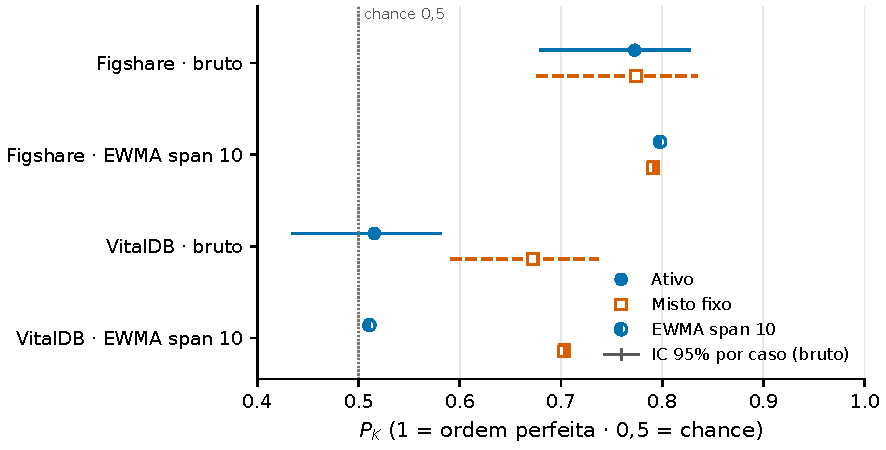
\includegraphics[width=0.90\columnwidth]{figures/pk_prediction.pdf}
\caption{Probabilidade de predição $P_K$, ativo vs.\ misto.}
\label{fig:pk}
\end{figure}

A leitura ordinal separa dois diagnósticos que o MAE sozinho confunde. No VitalDB o que se perde é a capacidade de ordenar, não a escala: o ativo erra 12,43 pontos sem ordenar melhor que o acaso, e o baseline espectral confirma o padrão (0,502). A recuperação parcial do misto (0,672) acompanha a exposição ao domínio, coerente com a leitura da Seção~\ref{sec:mae}. A concordância, a calibração e a incerteza detalhada ficam na Seção~\ref{sec:secundarias}.

\subsection{Implantabilidade: o custo da cadeia causal}
\label{sec:implantabilidade}

O melhor resultado publicado neste corpus vem de um TCN-BiLSTM com atenção de 1,07M de parâmetros, que sob GroupKFold por sujeito reporta 7,12 $\pm$ 0,42 brutos e 6,03 $\pm$ 0,38 após suavização, com CCC 0,819 \cite{sukriti2026}; a entropia amostral reportou 5,22 \cite{liu2018}. Este trabalho usa 0,15M de parâmetros e dez épocas de treino, e fica em 6,69--7,03 brutos, abaixo do bruto daquele modelo.

A comparação fica informativa quando se olha o que cada lado gastou para chegar lá. O TCN-BiLSTM escolhe o $\alpha$ do EWMA por MAE de validação, e no protocolo por sujeito ele recai com mais frequência em 0,05 ou 0,10: nesta convenção de \textit{span}, 19 a 39, ou seja de 45 a 95 s de idade média das amostras. O misto desta cadeia alcança o mesmo erro com 10 s, no span 5 (6,11; IC 95\% 4,84--7,96), e com 22,5 s, no span 10 (5,84; IC 95\% 4,56--7,62). O $\alpha = 0{,}35$, que casaria com o span 5 daqui, fica restrito às curvas de sensibilidade dos splits aleatórios.

A Figura~\ref{fig:ewma_tradeoff} posiciona a varredura contra esse referencial: toda ela cabe à esquerda da faixa em que ele opera. O span 10 não é a comparação principal porque dobra o atraso do span 5, de 10 s para 22,5 s, e o ganho além do span 5 é em parte emprestado da própria suavização.

\begin{table}[H]
\centering
\small
\setlength{\tabcolsep}{4pt}
\begin{tabular}{llrrrr}
\hline
Benchmark & Braço & Bruto & Span 5 & Span 10 & Span 15\\
\hline
Figshare & ativo & 7,03 & 6,38 & 6,10 & 5,91\\
Figshare & misto & 6,69 & 6,11 & 5,84 & 5,67\\
Figshare & RF espectral & 8,86 & 7,86 & 7,56 & 7,38\\
VitalDB & ativo & 12,43 & 12,11 & 12,06 & 12,06\\
VitalDB & misto & 8,60 & 7,95 & 7,89 & 7,93\\
VitalDB & RF espectral & 13,62 & 12,75 & 12,62 & 12,58\\
\hline
\end{tabular}
\caption{Efeito do EWMA causal por caso; MAE em pontos BIS; predições congeladas, sem retreino.}
\label{tab:ewma}
\end{table}

\begin{figure}[H]
\centering
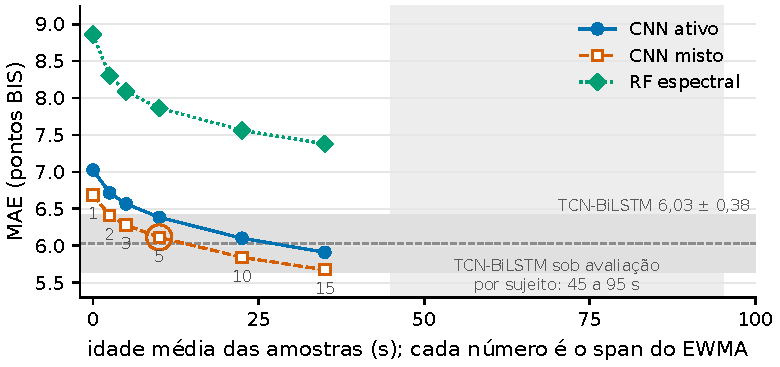
\includegraphics[width=0.88\columnwidth]{figures/ewma_tradeoff.pdf}
\caption{Compromisso entre atraso e erro no Figshare. Cada ponto é um span do EWMA causal, posicionado pela idade média das amostras e rotulado pelo span; a faixa cinza é o intervalo de erro que o TCN-BiLSTM reporta ($\pm 0{,}38$) e a linha tracejada, o ponto estimado dele. A região clara à direita é a faixa de atraso em que ele opera sob avaliação por sujeito ($\alpha$ de 0,05 a 0,10, isto é, de 45 a 95 s), e o anel marca o span 5 desta cadeia, com 10 s.}
\label{fig:ewma_tradeoff}
\end{figure}

A comparação é de ordem de grandeza, não de ranking: os protocolos diferem em normalização, seleção da suavização, agregação e medida de acordo. O que ela sustenta é o custo da cadeia: a suavização é uma recursão de uma linha ($s_t = \alpha y_t + (1-\alpha)s_{t-1}$) sobre predições congeladas, o filtro mantém estado causal por caso e o replay roda em CPU. Nenhum passo exige retreino, GPU ou acesso ao futuro, o que torna a cadeia candidata a uso ao vivo; já o modelo contemporâneo, com BiLSTM bidirecional e filtro de fase zero, não é estritamente causal \cite{sukriti2026}.

A Tabela~\ref{tab:ewma} mostra que o ganho é maior onde há ordenação para preservar: no Figshare o misto vai de 6,69 a 5,84; no VitalDB ativo o erro quase não muda (12,43 para 12,06) e o $P_K$ segue no acaso (0,515 para 0,511), o que reforça que ali o problema é de ordenação, não de ruído. Parte do ganho é esperada, pois o alvo é autocorrelacionado e o baseline espectral também melhora; a varredura é retrospectiva e exploratória.

\subsection{Análises secundárias e exploratórias}
\label{sec:secundarias}
\label{sec:fatorial}

O experimento fatorial fecha o diagnóstico da Seção~\ref{sec:mae}. Quatro braços foram treinados do zero no Figshare (mesmo split 13/5/5, seed 42, sem tocar nos checkpoints históricos): A (reprodução do baseline); B (A com winsorização causal $\pm200$ $\mu V$); C (B com perda de Huber $\delta=5$ e até 120 épocas); e D (C com z-score por sujeito, estimado no treino e congelado). Todos foram avaliados nos mesmos benchmarks.

O braço A reproduziu o histórico, validando o harness. O winsor isolado (B) piorou o Figshare, com viés negativo, sem mover o VitalDB. O treino longo com Huber (C) foi o único ganho interno real, com 46 épocas efetivas, mas não se sustenta no VitalDB. O z-score por sujeito (D) elevou Pearson e CCC no Figshare sem reduzir o MAE, e no VitalDB ficou perto dos demais. Nenhum braço moveu o transporte: todos ficaram entre 12,0 e 12,6, contra 8,60 do misto, que viu a fonte. O que separa os casos não é arquitetura, perda ou normalização, e sim a exposição ao domínio; o treino longo, aliás, aproxima esta cadeia da faixa publicada (6,63 contra 6,03 $\pm$ 0,38) sem resolver o transporte.

\begin{table}[H]
\centering
\footnotesize
\setlength{\tabcolsep}{3pt}
\begin{tabular}{llrrrr}
\hline
Benchmark & Braço & MAE (IC 95\%) & Pearson & CCC & $P_K$\\
\hline
Figshare & A (reprodução) & 7,03 (6,36--8,27) & 0,780 & 0,777 & 0,773\\
Figshare & B (winsor) & 8,19 (6,78--10,01) & 0,699 & 0,661 & 0,758\\
Figshare & C (Huber+longo) & 6,63 (6,03--7,67) & 0,824 & 0,820 & 0,780\\
Figshare & D (z por sujeito) & 7,14 (5,75--7,86) & 0,833 & 0,830 & 0,772\\
VitalDB & A (reprodução) & 12,64 (11,38--14,43) & 0,056 & 0,051 & 0,524\\
VitalDB & B (winsor) & 12,04 (10,89--13,74) & 0,238 & 0,194 & 0,528\\
VitalDB & C (Huber+longo) & 12,61 (11,40--14,22) & 0,145 & 0,134 & 0,553\\
VitalDB & D (z por sujeito) & 12,41 (11,35--13,67) & 0,185 & 0,168 & 0,536\\
\hline
\end{tabular}
\caption{Braços fatoriais novos (brutos, sem EWMA); MAE em pontos BIS; IC 95\% por bootstrap agrupado por caso; CCC é o coeficiente de Lin.}
\label{tab:fatorial}
\end{table}

A concordância e a calibração, exploratórias, seguem a mesma direção: a inclinação predito--referência cai de 0,72 no Figshare ativo para 0,02 no VitalDB ativo (ICC(2,1) 0,02; 57,2\% das janelas com $|erro|\leq10$); o misto recupera 0,55 no VitalDB e chega a 0,82 no Figshare (ICC 0,81; 80,6\%; Figura~\ref{fig:training}). O EWMA eleva o ICC do misto de 0,81 para 0,86 (Figshare) e de 0,67 para 0,71 (VitalDB).

O corpus tem 59 casos (33 elegíveis, 11 em quarentena e 15 VitalDB congelados; Figura~\ref{fig:corpus}).

\begin{figure}[tbp]
\centering
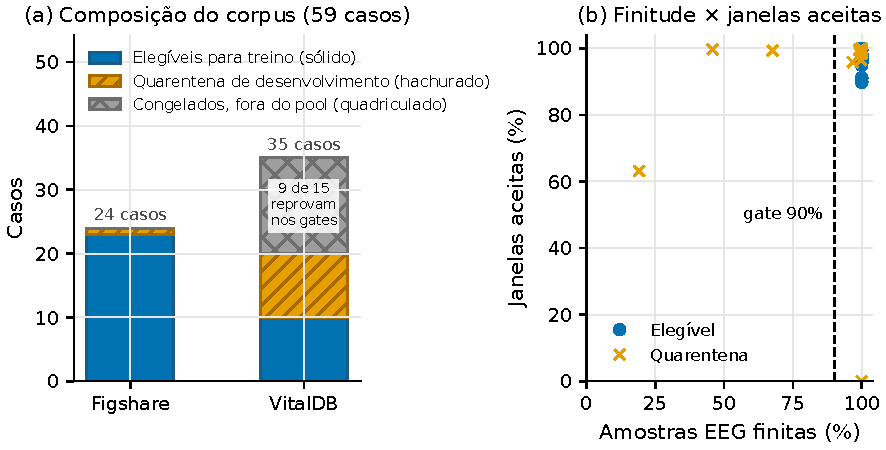
\includegraphics[width=0.95\columnwidth]{figures/corpus_panels.pdf}
\caption{Composição e qualidade do corpus (59 casos).}
\label{fig:corpus}
\end{figure}

\begin{figure}[tbp]
\centering
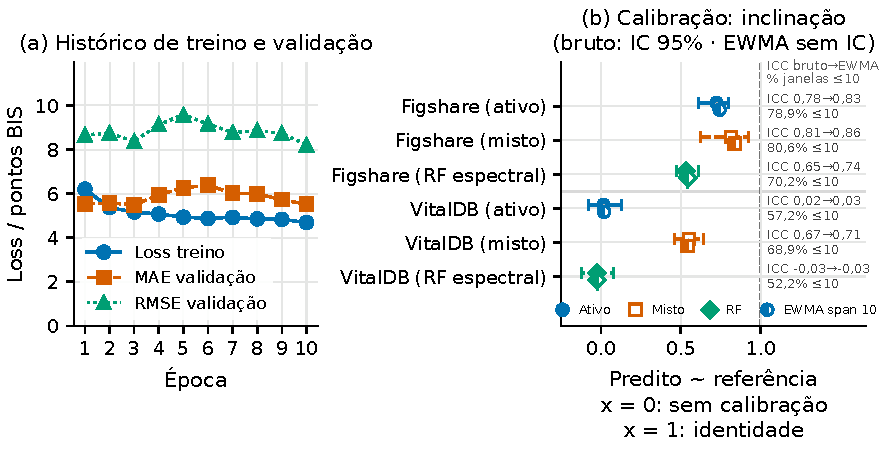
\includegraphics[width=0.95\columnwidth]{figures/training_panels.pdf}
\caption{Treinamento do ativo e calibração por braço.}
\label{fig:training}
\end{figure}

Os intervalos da Tabela~\ref{tab:benchmarks} vêm do bootstrap agrupado por caso ($B=1.000$, seed 42), cujas réplicas aparecem na Figura~\ref{fig:bootstrap}a,b. O intervalo do ativo no VitalDB cobre 0,5 em Pearson, coerente com a perda de ordenação já descrita; no Figshare, os intervalos de MAE do ativo e do misto se sobrepõem, o que sustenta a leitura de que a diferença ali não é sustentada. A grade de offset ($-20$ a $+20$ s, sem retreino, Figura~\ref{fig:bootstrap}c,d) mostrou o MAE variar de 7,22 a 6,76: tendência pós-hoc, sem valor causal e sem mudar o offset zero \cite{pilge2006}. A variação é pequena frente ao erro total: o alinhamento temporal do rótulo não explica a perda no VitalDB.

\begin{figure}[tbp]
\centering
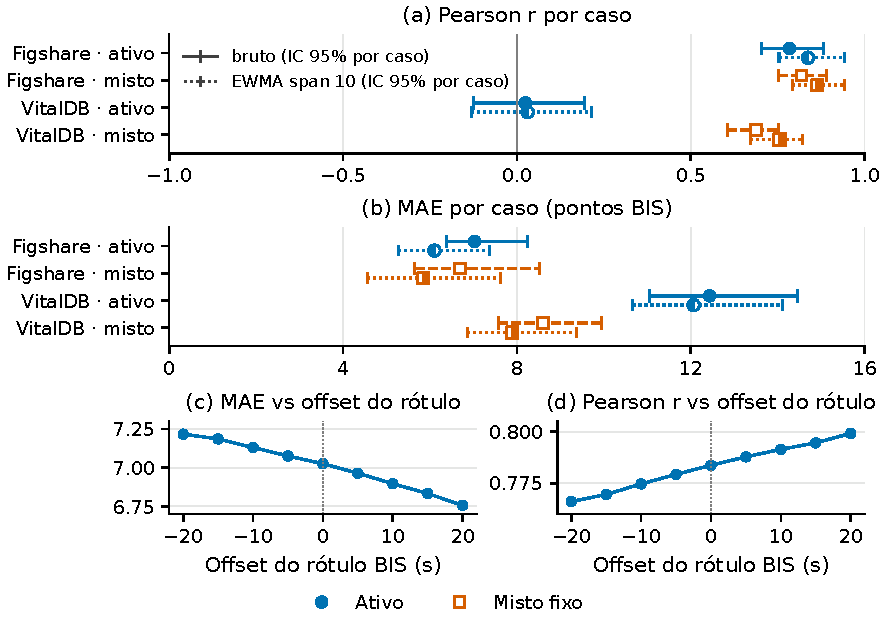
\includegraphics[width=0.92\columnwidth]{figures/bootstrap_offset.pdf}
\caption{Bootstrap agrupado por caso e sensibilidade ao offset do rótulo. (a,b) IC 95\% por caso, bruto e EWMA span 10. (c,d) Grade de offset $-20$ a $+20$ s, eixos ampliados (variação total $\leq 0{,}5$ ponto de MAE e $0{,}04$ de Pearson).}
\label{fig:bootstrap}
\end{figure}


\section{Discussão e limitações}

Três resultados delimitam este trabalho. Sob validação agrupada, uma CNN de 0,15M de parâmetros supera o controle espectral e ordena os momentos da cirurgia como a referência; com a suavização causal, ela alcança a faixa de erro do próprio monitor no corpus de origem, a um custo de execução que a mantém candidata a uso ao vivo; e esse desempenho não transporta para outra fonte. Os dois primeiros são o que o trabalho entrega; o terceiro delimita a alegação. A degradação do ativo do Figshare para o VitalDB é evidência de sensibilidade à troca de fonte, não prova de qual diferença a causou. A redução de erro do misto é compatível com adaptação após incorporar participantes VitalDB; como o benchmark é da mesma fonte e já havia sido observado, ele gera hipótese para uma nova coorte travada, não generalização externa \cite{lee2022,tripodai}. Nenhum treino restrito ao Figshare restaurou o transporte (Seção~\ref{sec:secundarias}): a exposição ao domínio, não a arquitetura ou a perda, explica o ganho do misto. A prioridade se desloca de ``modelo maior'' para ``dados da fonte'': o próximo passo é expor o treino a mais fontes, com partição travada e auditoria por hashes.

A melhora em 14/15 casos convive com piora no caso 16, e os agregados por janela privilegiam cirurgias longas. A referência de 10 unidades é escala de concordância entre medições do monitor, não limiar para MAE \cite{harada2021}. Para a validação futura, o desenho mínimo seria uma coorte travada de outra fonte, com partição por participante definida antes de qualquer inspeção, métricas primárias pré-registradas (MAE por janela e $P_K$) e relato de calibração; sem isso, qualquer novo candidato repete o estatuto exploratório deste trabalho \cite{tripodai,archer2021}.

Uma diferença operacional separa o benchmark do cenário de execução, e ela é de primeira ordem. Nos 15 casos VitalDB, a construção offline interpola valores não finitos, podendo usar amostras posteriores à janela, e interpola o BIS para uma grade de 1 s sem máscara persistida; o replay causal, ao contrário, rejeita a janela e nunca lê o futuro. Como a interpolação pode se apoiar em amostras indisponíveis no instante da emissão, os números VitalDB desta avaliação tendem a ser otimistas frente ao que um replay produziria; o tamanho da diferença não foi medido, e a construção foi mantida por fidelidade ao protocolo histórico.

O bootstrap cobre só a variabilidade de reamostrar os casos disponíveis; não cobre incerteza de treinamento, seleção de checkpoint, mudança de centro ou erro do rótulo. O pequeno $n$ Figshare e o reaproveitamento do benchmark VitalDB impedem leitura confirmatória \cite{field2007,archer2021}; a avaliação é pré-clínica.

O alvo é a saída BIS, sensível a EMG, bloqueio neuromuscular, cetamina e atrasos; baixo erro contra o monitor não equivale a medir consciência ou efeito farmacológico \cite{schuller2015,hans2005,pilge2006}. A banda de 0,5--45 Hz inclui gama frontal sensível a EMG, e o \textit{notch} fixo em 50 Hz pode não corresponder à rede de cada centro; nenhuma sensibilidade foi medida. Faixas e limiares de qualidade são heurísticas sem validação clínica; DOSE-I permanece tarefa separada \cite{dosei}.

% Quebra de linha local (sem alterar o texto).
\begingroup\emergencystretch=1em\relax A suavização EWMA é pós-hoc, com span escolhido após os resultados, e não substitui os números brutos da Tabela~\ref{tab:benchmarks}. A cadeia registra hashes, partições, pré-processamento e replay; a política de amostragem do checkpoint ativo não foi registrada, limitação histórica \cite{tripodai}.
\par\endgroup

\section{Conclusão}

O BrainSniffer entrega uma cadeia compacta, causal e auditável para estimar a referência BIS a partir de EEG frontal. Com 0,15 milhão de parâmetros, dez épocas de treino e execução em CPU, o checkpoint ativo superou o controle espectral sob validação agrupada (MAE 7,03 contra 8,86; $\Delta$ pareado $-1{,}84$) e ordenou os momentos da cirurgia como a referência ($P_K$ 0,773). Com uma suavização causal de uma linha sobre as predições congeladas, sem retreino, o misto chega à mesma ordem de grandeza do melhor resultado publicado neste corpus: no span 5, com 10 s de atraso, alcança 6,11 contra os 6,03 $\pm$ 0,38 do TCN-BiLSTM de 2026, que usa cerca de sete vezes mais parâmetros, memória de 45 a 95 s e um filtro de fase zero que não existe ao vivo. Os protocolos diferem, e o span 5 foi escolhido após ver os resultados, logo não é um ranking. O erro fica abaixo da escala de leitura de 10 pontos \cite{harada2021}, o que motiva avaliação prospectiva da cadeia; não demonstra equivalência, aceitabilidade clínica ou não-inferioridade.

O limite é claro e está declarado ao longo do texto: o desempenho não transporta para outra fonte. No VitalDB o ativo perde a ordenação ($P_K$ 0,515, indistinguível do acaso) e erra 12,43, e o misto melhora 14 dos 15 casos apenas após ver essa fonte, o que é adaptação ao domínio, não generalização. O experimento fatorial mostra que nenhum treino restrito ao Figshare fecha essa diferença, o que desloca a prioridade de ``modelo maior'' para ``dados da fonte''. Quanto à reprodutibilidade, o braço A reconstrói o checkpoint ativo a partir da configuração documentada, com os mesmos números no Figshare; o registro da política de amostragem da execução histórica não foi preservado, então ela vale para a cadeia, não para o checkpoint original \cite{tripodai}.

Os resultados são retrospectivos e exploratórios, e limitados pelo rótulo, pelos casos, pelo reuso dos benchmarks e pela imputação offline. A contribuição defensável é uma base auditável para formular e testar hipóteses, não um sistema clínico: o software não mede consciência, não prescreve dose, não controla bomba e não deve acionar alarme ou conduta.

\subsection*{Disponibilidade}
Código em \url{https://github.com/Bruno-BRG/brainsniffer} (MIT); dados não redistribuídos; relatórios com hashes.

\begin{small}
\bibliographystyle{sbc}
\bibliography{referencias}
\end{small}

\end{document}
